\section{System Development}

After concluding the research portion of the Thesis there will be a clear set of goals for L2 pedagogy, vowel space measurement, and visual feedback strategies. With these goals taken into account, the CAPT tool for training German vowel perception and production will be implemented. The tool will be based on a concept from \citep{Carroll2015}, but will be re-factored from a Praat Script program into a Java application and be given improved functionality. 

\subsection{System Functionality}
The previous system was designed to identify a single vowel from a recording of a monosyllabic word and measure formant values and duration information to be rendered as visual feedback. The visual feedback for spectral information was rendered as a point in a 2 dimensional plane, and the user was also provided model German productions and target areas in the 2D plan to try and emulate.  As mentioned earlier when discussing describing the vowel space, this representation of large vowel category targets represents the most basic case of vowel feedback.  In order to improve the vowel specific feedback, the revised version of the CAPT tool will first take a measurement of each user's  cardinal vowels (example: \textipa{i, u, A}) and 


This is done by looking at the intensity curve of the recording and selecting the part of the signal which is within 10 dB of peak intensity and which has a duration of at least 40 ms (see figure \ref{fig:intensity}). This approach is a rather naive means of identifying the vowel\footnote{For the purposes of prototype development, this method of vowel identification has been effective, however future improvements will be proposed in the following section.}, and relies on the assumption that the vowel will be the most sonorant segment of the utterance and have a relatively long duration. Therefore, in order to control for better vowel identification, all nonsense words used in the training are monosyllabic monophthongs which have short duration, low intensity consonants preceding and following the vowel. After the vowel boundaries have been established, duration is easily calculated, as well as a midpoint for the vowel. From the midpoint automatic measurements of the 1st and 2nd formants are made using a Praat formant object.

\begin{figure}[H]
 \centering
 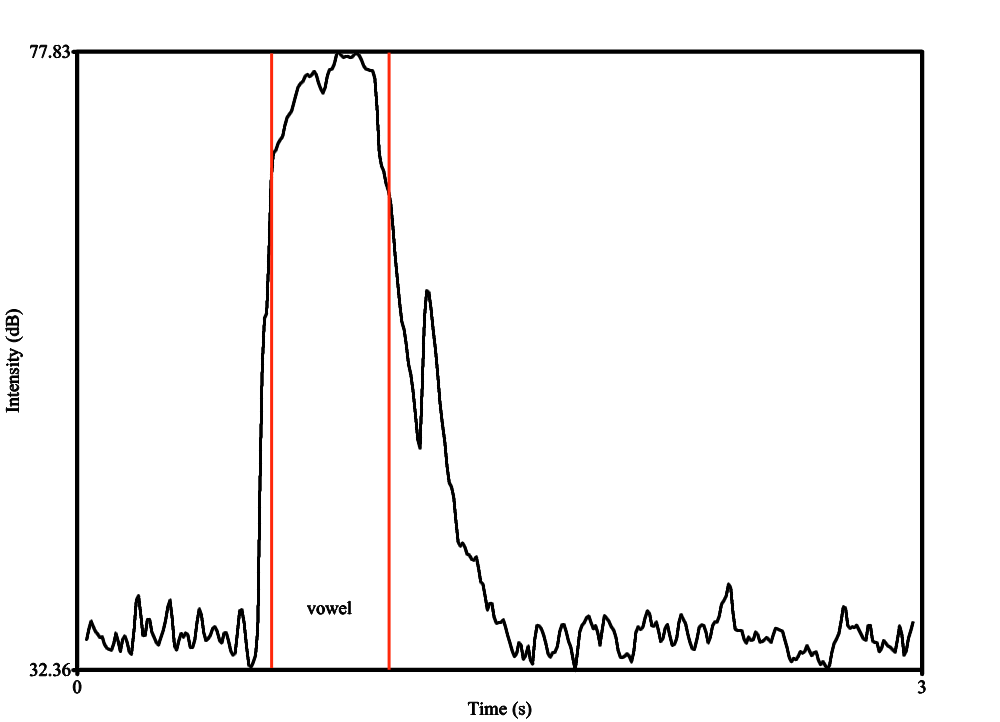
\includegraphics[scale=1.2]{intensity_for_paper.png}
 \caption{Selecting the region with peak intensity (Max dB to Max dB -10) as the vowel region.}
 \label{fig:intensity}
\end{figure}

With the duration and formant information, the script calls a function to plot a point in the acoustic space and draw a duration bar. The same algorithm is used for both the user input, as well as pre-recorded native German input for the sake of consistency. Previous user recordings are also stored for playback, and the buttons in the bottom right side of the UI are updated to reflect the most recent recordings.


\subsection{System Layout}
The region in the bottom left side of the figure (label 1) contains buttons which play back examples of minimal pair nonsense words spoken by a native German speaker. When a sound has been played, two modes of visual feedback are provided to show the listener some of the the qualities of the vowel produced. Spectral information is provided by plotting a point representing the F1-and F2-values of the vowel superimposed on set of targets in acoustic space.  The duration of the vowel is displayed to the right in green. The user can then attempt their own production of the nonsense word, after which, the audio is processed and the vowel is plotted in the acoustic space and as a duration bar. Both the plotted point, and the duration bar appear in red and are labeled ``user'' so that the user can see how their production of the vowel compares to the native German pronunciations labeled in green. the user can see if new attempts at producing the vowels are getting closer to the targets. The user may also listen to the previous 5 recordings they have produced (label 3) in order to sensitize their ear to the subtle changes in vowel quality which produced different results.


\begin{figure}[H]
 \centering
 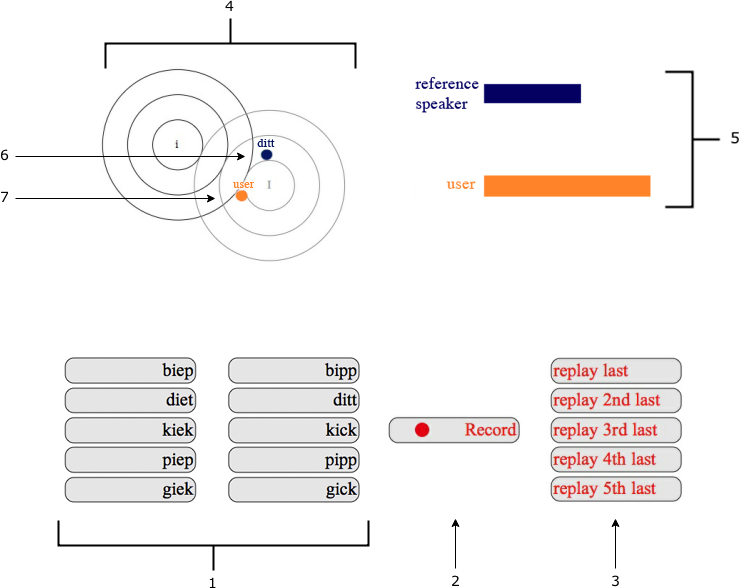
\includegraphics[scale=.42]{ui2.png}
 \caption{User Interface with the numbered regions showing the following: 1: playback of native speaker, 2: record button, 3: playback of user, 4; acoustic space with vowel targets, 5: duration space with vowel lengths from native speaker and user, 6 \& 7: vowels from native speaker and user plotted in acoustic space.}
 \label{fig:ui}
\end{figure}







%Because vowels are difficult to describe in terms of clearly defined articulatory positions, we have opted to adopt an abstract visual approach to feedback which shows the vowel's acoustic characteristics in two-dimensional space, and the duration as a bar graph. By drawing these features, the user has a visual analogy of what happening in the vowel, and can use that as a supplementary source of information when training vowel production.
